\documentclass[a4paper,12pt]{article} % тип документа
\usepackage[margin=1in]{geometry} % Поля

%  Русский язык
\usepackage[warn]{mathtext}
\usepackage[T2A]{fontenc}			% кодировка
\usepackage[utf8]{inputenc}			% кодировка исходного текста
\usepackage[english,russian]{babel}	% локализация и переносы
% Математика
\usepackage{amsmath,amsfonts,amssymb,amsthm,mathtools} 
\usepackage{wasysym}
%%%
\usepackage{graphicx}
\usepackage{svg}

\usepackage{tabularx}

\usepackage{gensymb} % знак градуса
\usepackage{enumitem} % изменить список enumerate
\usepackage{placeins} % \FloatBarrier

\renewcommand{\thesection}{\Roman{section}} 
\renewcommand{\thesubsection}{\roman{subsection}}


\begin{document}

\newcolumntype{Y}{>{\centering\arraybackslash}X} %new tabularx


%титул
\hrule 	
\medskip
\begin{raggedright}
{\large \textbf{Отчёт по работе 5.2.3}}
\\
\medskip
{\Large Интерферометр Рэлея} 
\\
\medskip
{\large Карташов Констанин Б04-005}
\medskip
\hrule
\medskip
\end{raggedright}


\section{Анотация}

\paragraph{Цель работы:} 
Ознакомление с интерференцией на двух щелях, устройством и принципом действия интерферометра Рэлея и с его применением для измерения показателей преломления газов.

\paragraph{Оборудование:}
\begin{itemize}
\renewcommand{\labelitemi}{$\triangleright$}
\itemsep-0.5em
\item технический интерферометр ИТР-1
\item светофильтр
\item баллон с углекислым газом
\item сильфон
\item манометр
\item краны
\end{itemize}


\medskip\hrule\medskip
\FloatBarrier
\section{Теоретическая часть}


\subsection{Устройство установки}

\begin{figure}
\centering
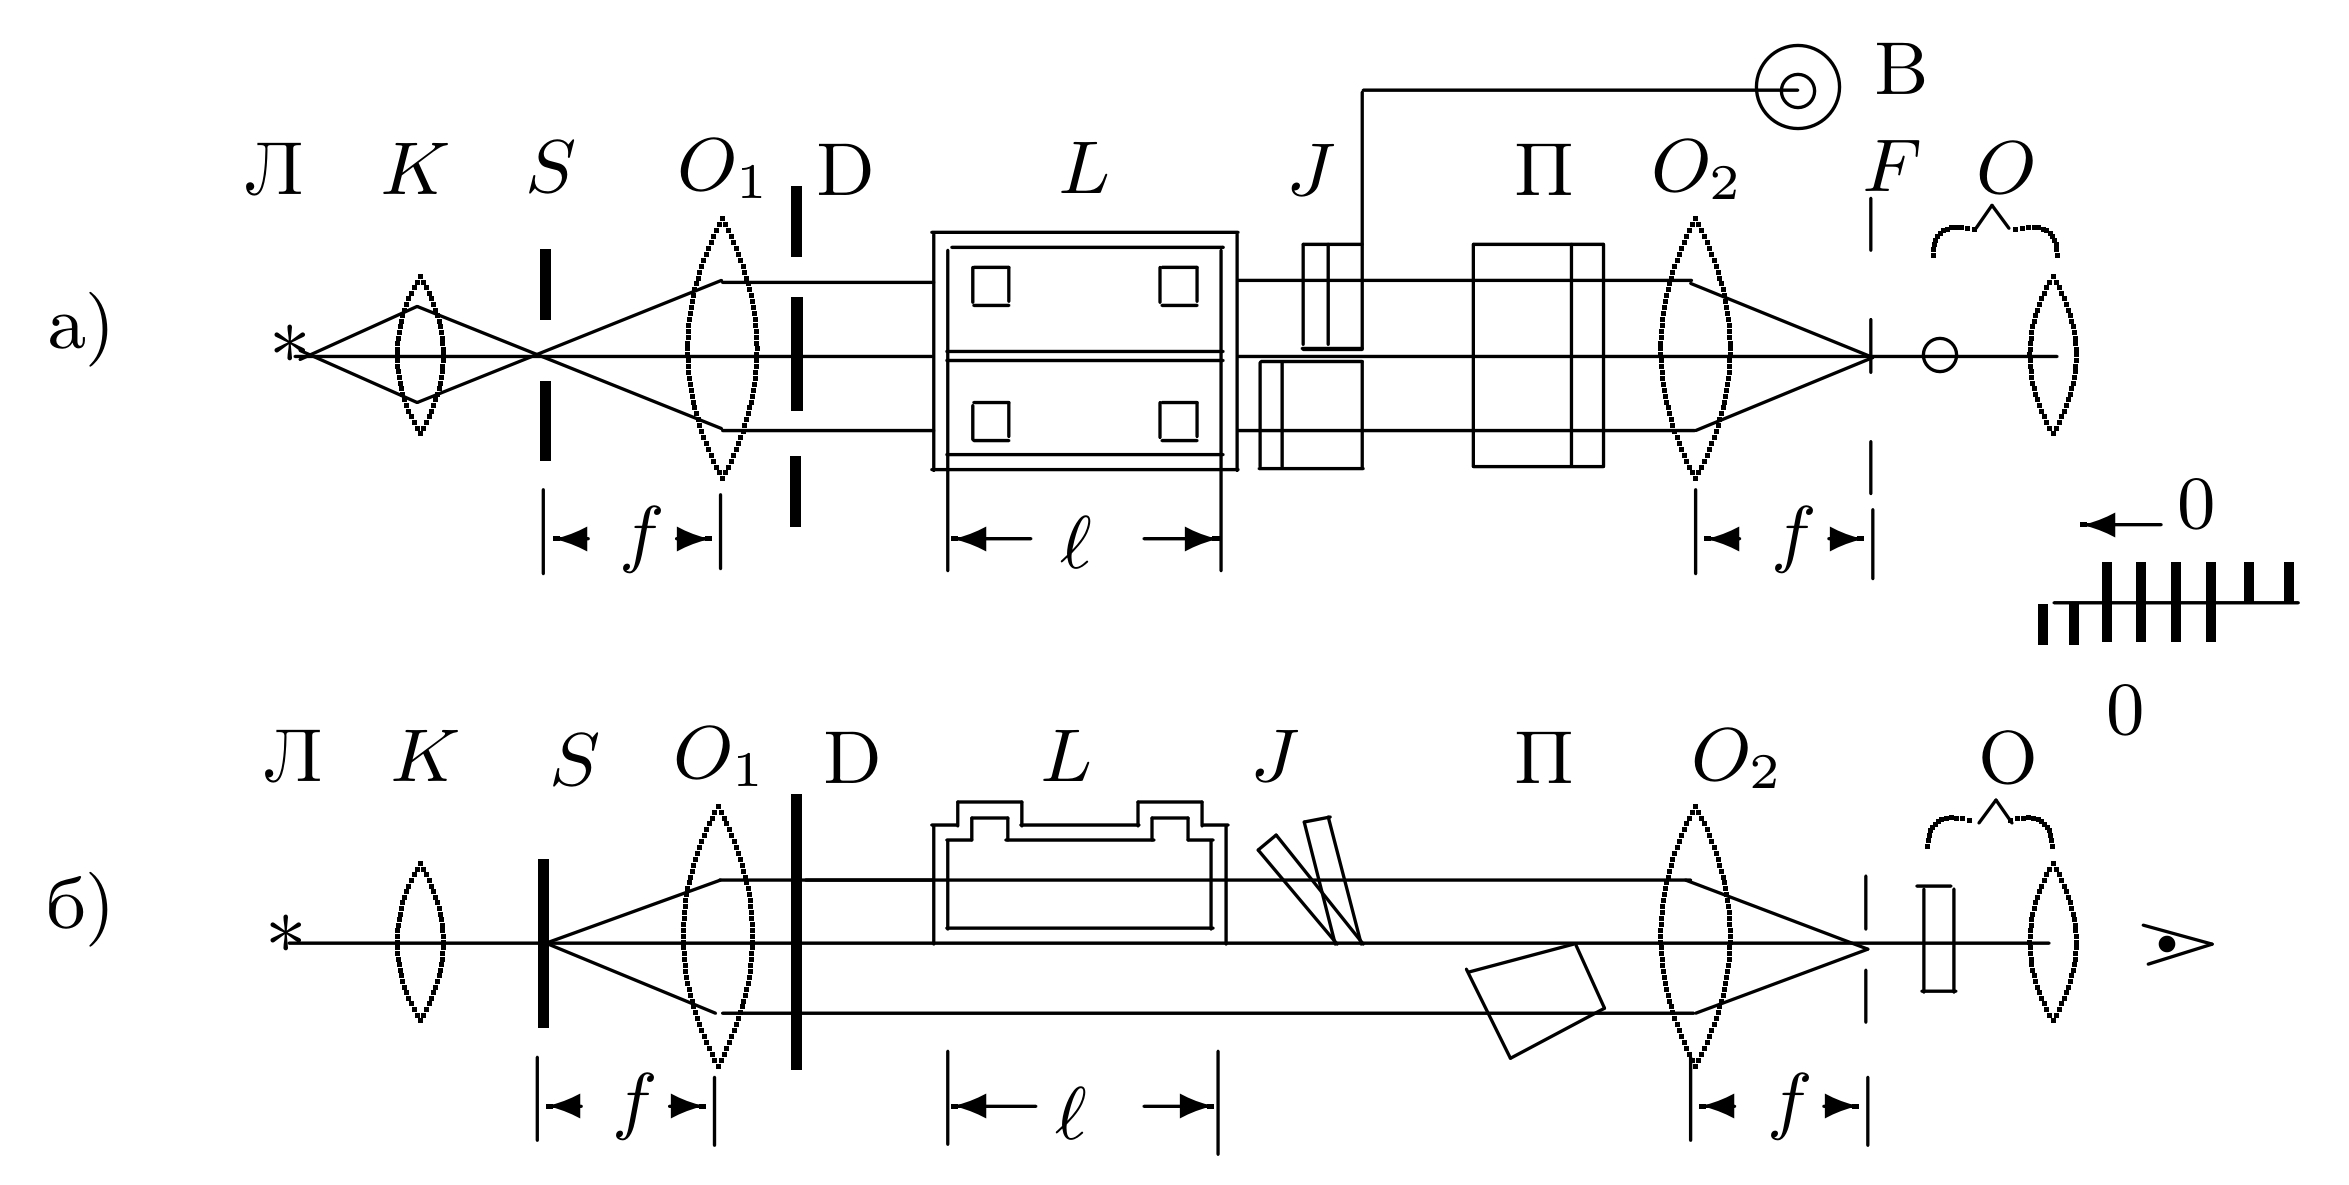
\includegraphics[width=0.8\textwidth]{setup.jpg}
\caption{Устройство интерферометра Рэлея: а) вид сверху; б) вид сбоку}
\label{f:setup}
\end{figure}

\paragraph{} Интерферометр Рэлея -- прибор для измерения разности показателей преломления, основанный на явлении дифракции света на двух параллельных щелях. Схема прибора представлена на рис. \ref{f:setup}. Лампа накаливания Л с помощью конденсора К освещает узкую входную щель S, расположенную в фокусе объектива О$_1$. Коллиматор состоящий из щели S и объектива О$_1$, посылает параллельный пучок на диафрагму D с двумя вертикальными щелями. Свет после двойной щели проходит кювету L, состоящую из двух одинаковых стеклянных камер, в которые вводятся исследуемые газы. Кювета анимает только верхнюю часть пространства между объективами О$_1$ и О$_2$, длина кюветы $l$. За кюветой расположены две стеклянные пластины J и пластинка П.

\paragraph{} Интерференционная картина наблюдаемая в объектива интерферометра, проедставляет собой две система равноотстоящий полос, параллельных щелям: верхняя (подвижная) образована лучами, прошедшими через кюветы, нижняя (неподвижная) образована лучами прошедшими под ними.

\paragraph{} При малых дифракционных углах $\varphi = \lambda/d$ расстояние между соседними светлыми (или тёмными) полосами $\delta y$ зависит от длины волны $\lambda$, фокусного расстояния $f$ объектива О$_2$ и расстояния между дифракционными щелями $d$:

\begin{equation}
\delta y = f \frac{\lambda}{d}.
\label{e:difr}
\end{equation}

\paragraph{} При заполнении камер газами с одинаковым показателем преломления обе системы полос совпадают. Оптическая разность хода $\Delta = \delta n \cdot l$, возникающая при прохождении света через камеры с разными газами $\delta n = n_2 - n_1$, ведёт к поперечному смещению верхней дифракционной картины относительно нижней. Смещение на одну полосу соответствует дополнительной разности хода $\Delta = \lambda$. Посчитав число полос $m$ между центрами обех картин, можно рассчитать

\begin{equation}
\delta n = \frac{\Delta}{l} = m \frac{\lambda}{l}.
\label{e:deltan}
\end{equation}

Показатель преломления $n$ исследуемого газа определяется путём сравнения с воздухом при атмосферном давлении:

\begin{equation}
n = n_\text{возд} + \frac{\Delta}{l}.
\label{e:air}
\end{equation}

Величина $\Delta$ определяется из смещения положения компенсатора J. Для этого компенсатор следует откалибровать.

\subsection{Зависимость показателя преломления газа от давления и температуры.}

\paragraph{} Диэлектрическая проницаемость $\varepsilon$ газа невзаимодействующих диполей, считается по формуле:

\begin{equation}
\varepsilon = n^2 = 1 + N\alpha,
\label{e:eps}
\end{equation}

\noindent где $N$ -- концентрация молекул, $\alpha$ -- поляризуемость молекулы (в СИ). Эта формула справедлива для разрежённых газов, и их коэффициент преломления мало отличается от единицы. Учитывая зависимость давления $P$ газа от температуры $P = NkT$, где $k$ -- постоянная Больцмана, получим соотношение
\[
n - 1 \approx \frac{\alpha}{2kT}P.
\]
\noindent Тогда для разности показателей преломления $\delta n$, измеряемой с помощью интерферометра Рэлея, и разности давления $\delta P$, измеряемой с помощью манометра, имеем простое соотношения:

\begin{equation}
\delta n = \frac{\alpha}{2kT}\delta P, \;\;\; \left. \frac{\partial n}{\partial P} \right|_{T = \operatorname{const}} = \frac{\alpha}{2kT}.
\label{e:part}
\end{equation}

\medskip\hrule\medskip
\FloatBarrier
\section{Экспериментальная часть}

\paragraph{Параметры установки}

\begin{itemize}
\renewcommand{\labelitemi}{$\triangleright$}
\item Длина кюветы $l = 25$ см
\item Длина волны пропускаемая фильтром $\lambda = 670 \pm 50$ нм
\item Температура воздуха $T = 23\degree \text{C} = 296$ К
\item Атмосферное давление $P = 99.6$ кПа
\end{itemize}

\subsection{Калибровка компенсатора}

\paragraph{} В обеих кюветах находится воздух при атмосферном давлении и при одинаковой температуре. Совместим центральные полосы дифракционных картин и зафиксируем соответствующее показание компенсатора $z$ -- оно будет нулевым. Теперь будем смещать дифракционную картину на целое число полос $m$ влево и вправо и фиксировать соответствующие показания компенсатора (табл. \ref{t:cal}). По полученным точкам построим калибровочную прямую методом наименьших квадратов (рис. \ref{f:cal}). 

\begin{table}
\centering
\begin{tabular}{|c|c|c|c|c|c|c|c|c|}
\hline 
$m$ & -7 & -6 & -5 & -4 & -3 & -2 & -1 & 0\\
\hline
$z$ & 17 & 48 & 79 & 117 & 153 & 185 & 220 & 261\\
\hline
$m$ & 0 & 1 & 2 & 3 & 4 & 5 & 6 & 7\\
\hline
$z$ & 261 & 296 & 331 & 364 & 401 & 437 & 472 & 501\\
\hline 
\end{tabular} 
\caption{Данные для калибровки компенсатора}
\label{t:cal}
\end{table}

\begin{figure}
\centering
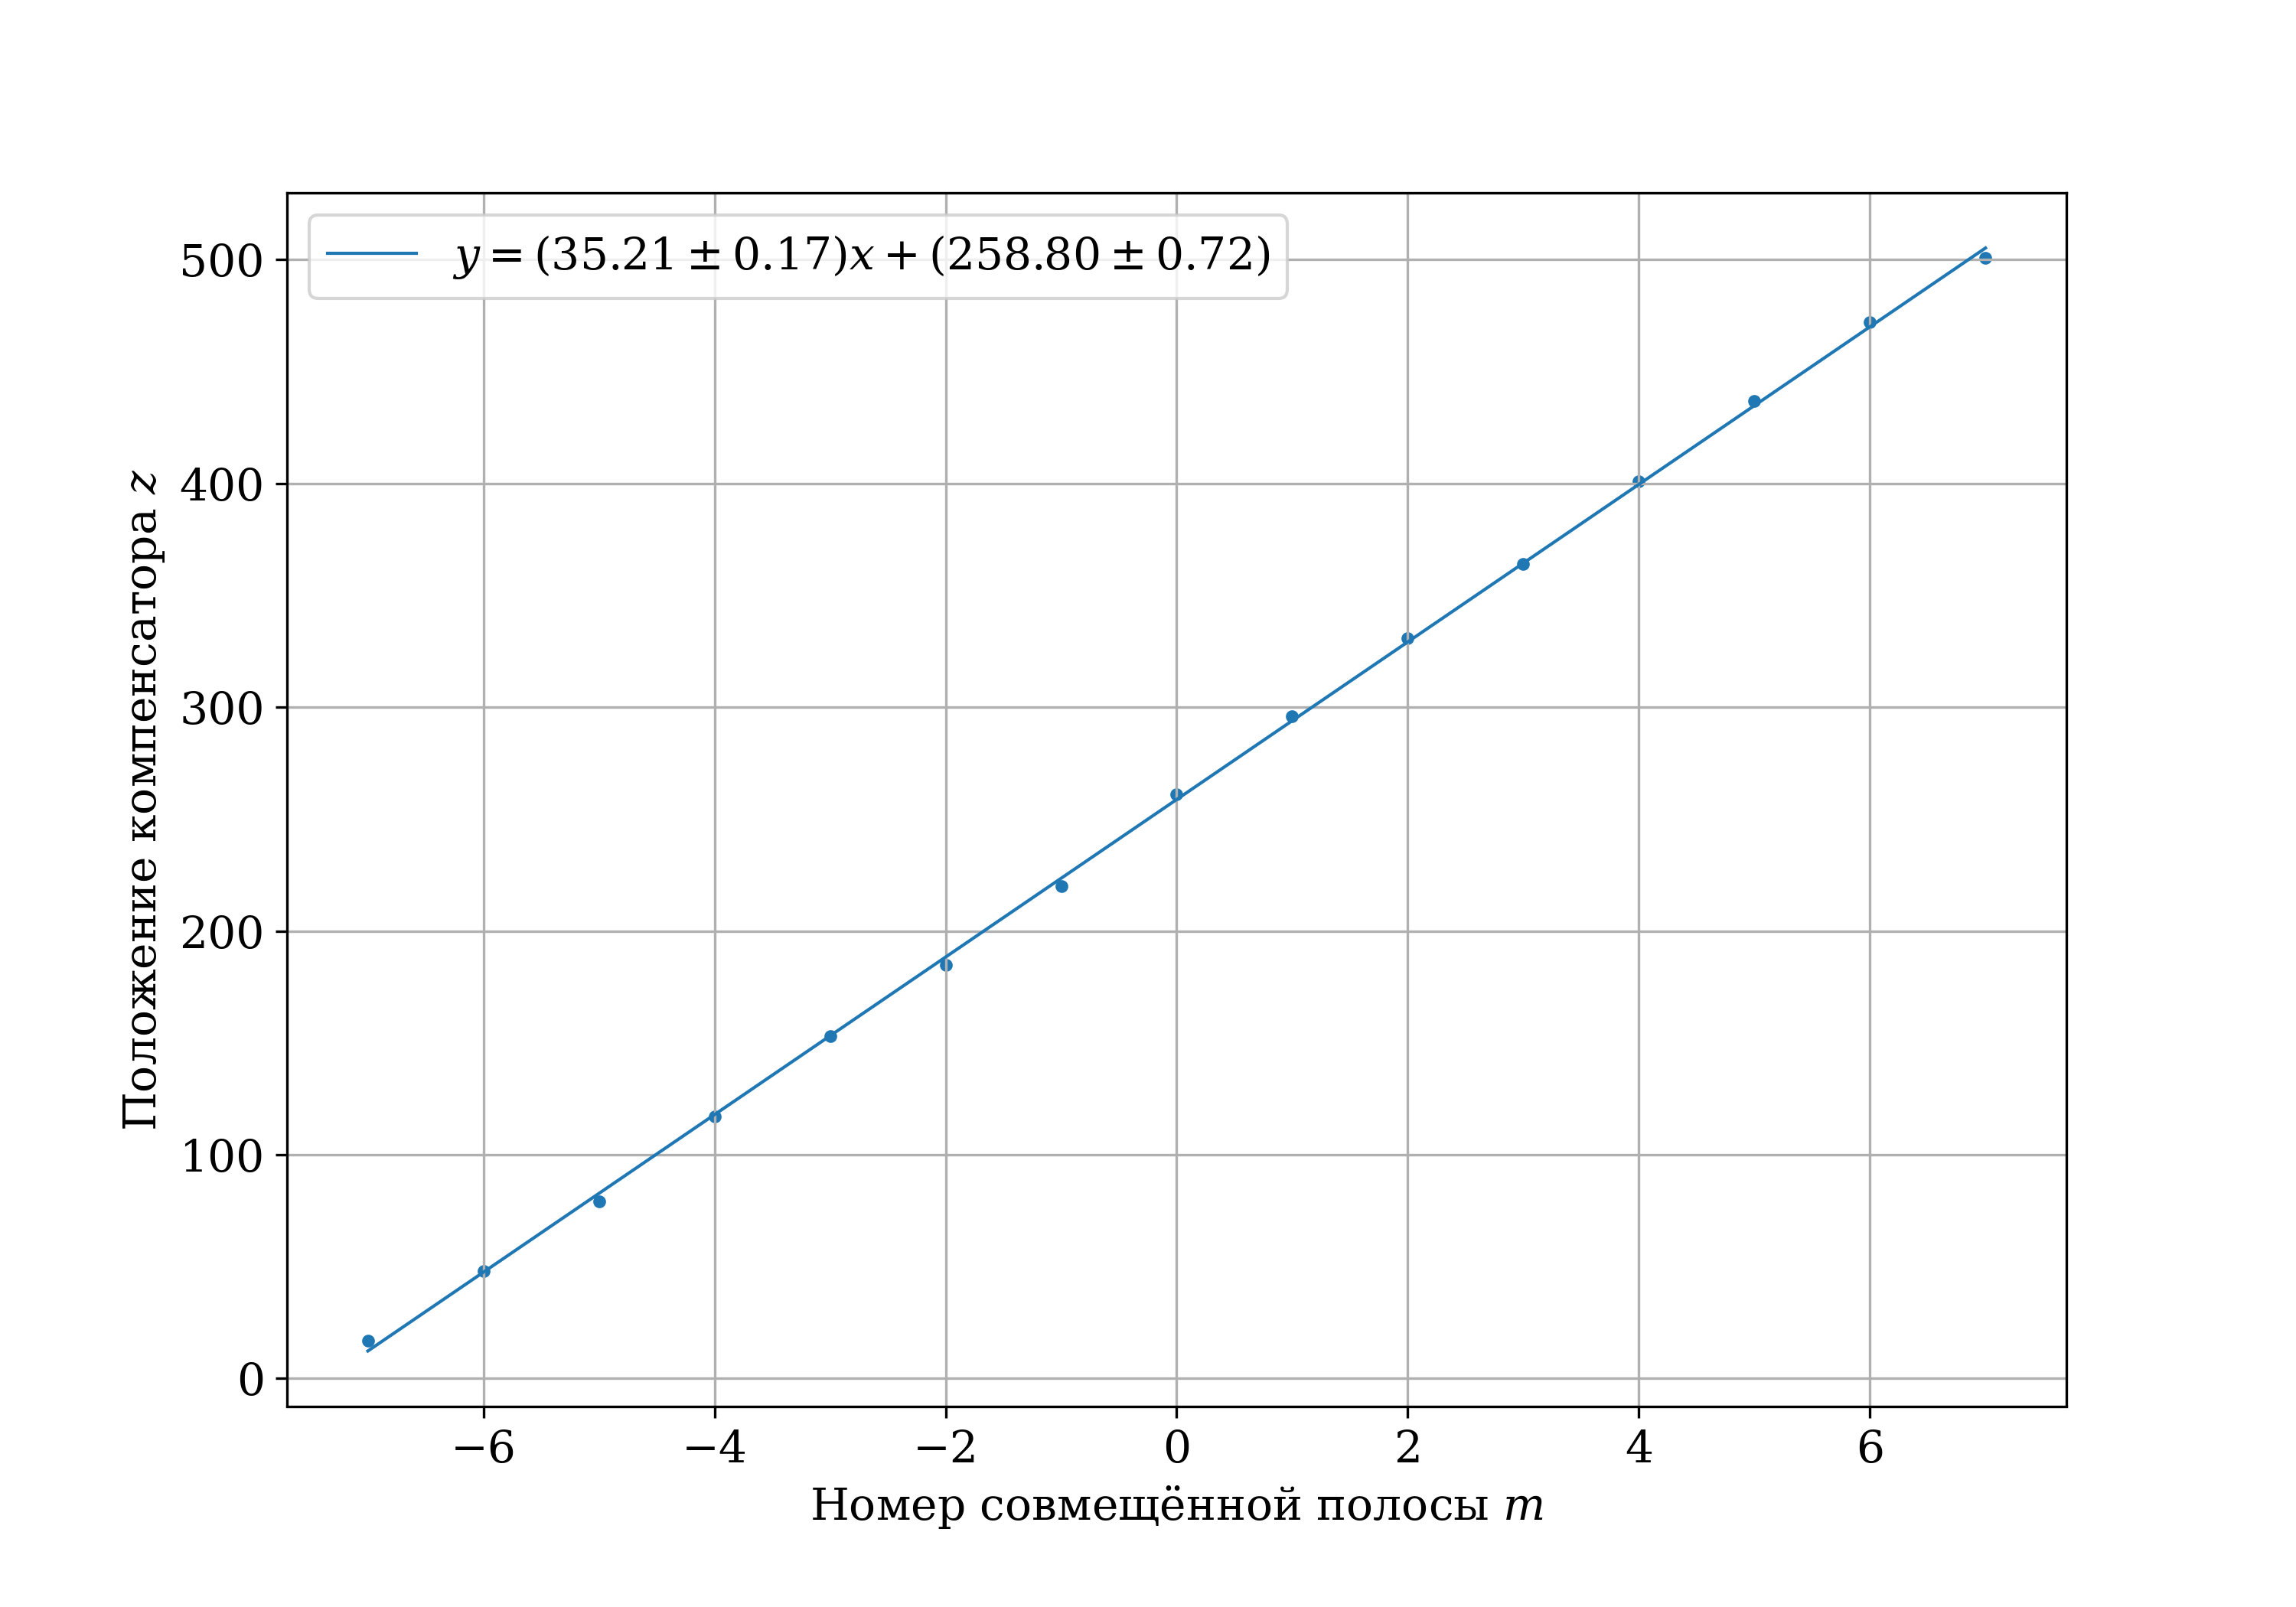
\includegraphics[width=\textwidth]{plot1.png}
\caption{Калибровочная прямая компенсатора}
\label{f:cal}
\end{figure}

\paragraph{} Случайная погрешность проведённой прямой оказалась достаточно малой $\varepsilon \approx 0.5 \%$. Поэтому в качестве систематической погрешности измерения разности хода будет брать длину волны фильтра, так как в дальнейших измерения происходит постоянное смещение дифракционной картины, и точное смещение полос не является возможным ($\Delta \Delta_\text{сист} = \lambda$).

\subsection{Зависимость показателя преломления воздуха от давления}

\paragraph{} В одной из кювет находится воздух под атмосферным давлением, в другой воздух под давлением. Будем менять давление в пределах от $-1000$ до $1000$ мм вод. ст. и смещать центральные полосы для каждого значения давлений, в процессе фиксируя положение компенсатора соответствующее значению давления. Далее по калибровочному графику рассчитаем разность хода, и по формуле (\ref{e:deltan}) найдём соответствующею величину $\delta n$. Все измеренные и полученные величины записаны в табл. 

\begin{table}
\centering
\footnotesize
\begin{tabular}{|c|c|c|c|c|c|c|c|c|c|c|}
\hline 
$\Delta P$, мм вод.ст. & -1000 & -900 & -800 & -700 & -600 & -500 & -400 & -300 & -200 & -100\\
\hline
$\Delta P$, Па & -9800 & -8820 & -7840 & -6860 & -5880 & -4900 & -3920 & -2940 & -1960 & -980\\
\hline
$z$ & 632 & 577 & 540 & 500 & 457 & 422 & 386 & 356 & 322 & 281\\
\hline
$\delta n \cdot 10^6$ & 28.4 & 24.21 & 21.4 & 18.35 & 15.08 & 12.42 & 9.68 & 7.4 & 4.81 & 1.69\\
\hline
$\Delta P$, мм вод.ст. & 100 & 200 & 300 & 400 & 500 & 600 & 700 & 800 & 900 & 1000\\
\hline
$\Delta P$, Па & 980 & 1960 & 2940 & 3920 & 4900 & 5880 & 6860 & 7840 & 8820 & 9800\\
\hline
$z$ & 210 & 182 & 150 & 116 & 90 & 46 & 9 & -26 & -54 & -100\\
\hline
$\delta n \cdot 10^6$ & -3.71 & -5.84 & -8.28 & -10.87 & -12.84 & -16.19 & -19.01 & -21.67 & -23.8 & -27.3\\
\hline
\end{tabular} 
\caption{Данные для построения зависимости $\delta n (P)$}
\label{t:pres}
\end{table}

По данным из табл. \ref{t:pres} построим график с погрешностями $\Delta \delta n = \Delta \Delta_\text{сист} / l = 2.68 \cdot 10^{-6}$ (из формулы \ref{e:deltan}) и $\Delta \Delta P = 50$ мм вод.ст. $\approx 500$ Па из-за необходимости постоянно поддерживать давление вручную. Видим, что одно значение сильно выбивается на фоне остальных (выделено оранжевым крестом), оно будет исключено из дальнейших расчётов. По методу наименьших квадратов проведём прямую через точки (рис. \ref{f:pres}).

\begin{figure}
\centering
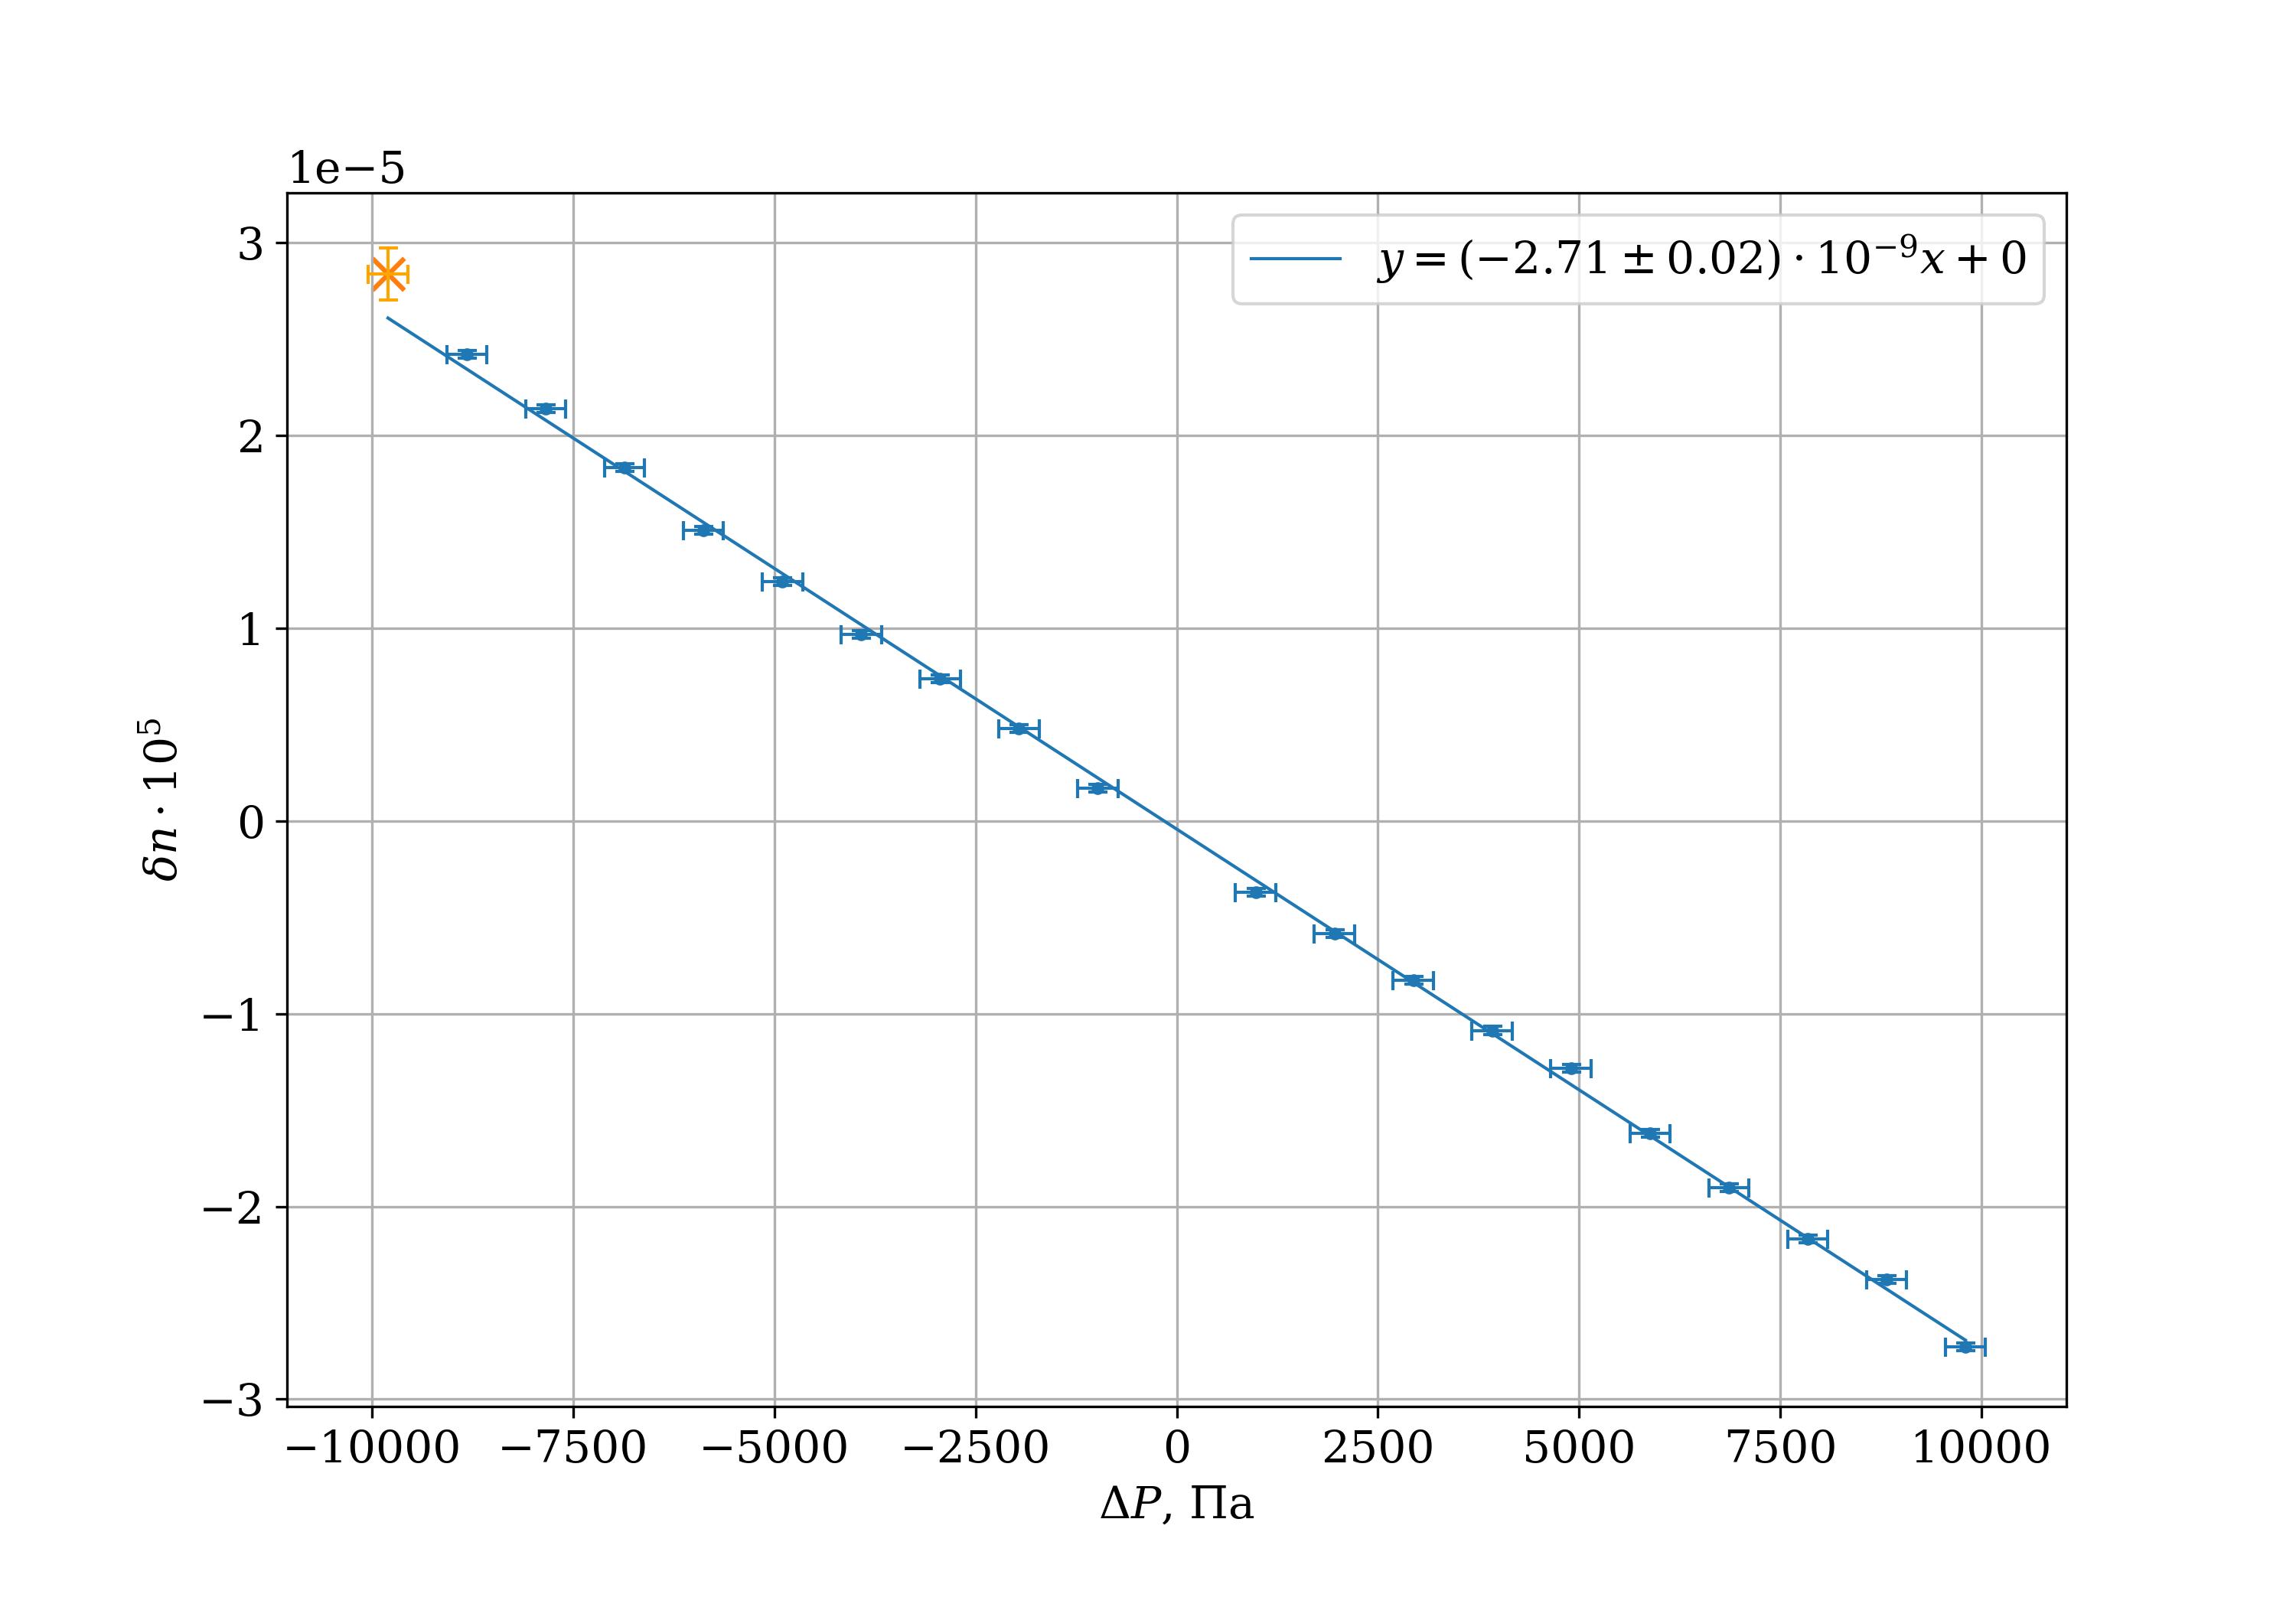
\includegraphics[width=\textwidth]{plot2.png}
\caption{График зависимости показателя преломления от давления}
\label{f:pres}
\end{figure}

\paragraph{} Полученное по методу наименьших квадратов значение $\delta n / \delta P = (-2.71 \pm 0.02) \cdot 10^{-9}$. Из теоретической части следует, что это значение должно быть положительным (формула (\ref{e:eps})), поэтому мы можем сделать вывод, что калибровочный график должен быть развёрнут относительно оси ординат. Берём значение $\delta n / \delta P = 2.71$. Систематическая погрешность $\varepsilon_\text{сист} = \sqrt{\left(\frac{\Delta \Delta P}{\Delta P} \right)^2 + \left(\frac{\Delta \delta n}{\delta n} \right)^2}$. Эта погрешность определяется крайними точками через которые проводится прямая, т.е $\varepsilon_\text{сист} = \sqrt{\left(\frac{500}{10000} \right)^2 + \left(\frac{2.6}{28} \right)^2} \approx 10 \%$ -- относительная погрешность коэффициента наклона графика. Поэтому $\delta n / \delta P = (2.7 \pm 0.3) \cdot 10^{-9}$.

\paragraph{} По формуле (\ref{e:difr}) найдём среднею поляризацию молекул воздуха:
\[
\alpha = 2kT \frac{\delta n}{\delta P} = 2 \cdot 1.38 \cdot 10^{-23} \cdot 296 \cdot 2.7 \cdot 10^{-9} \approx (2.2 \pm 0.2) \cdot 10^{-29} \; \text{Кл}\cdot\text{м}.
\]
\paragraph{} По формуле (\ref{e:eps}) найдём коэффициент преломления воздуха:
\[
n = \sqrt{1 + N \alpha} = \sqrt{1 + 2 P \frac{\delta n}{\delta P}} \approx 1 + P \frac{\delta n}{\delta P} = 1 + \cdot 10^5 \cdot 2.7 \cdot 10^{-9} \approx 1.00027 \pm 0.0003.
\]

\noindent Полученное значения для показателя преломления воздуха содержит в своей погрешности табличное значение данной величины.

\subsection{Показатель преломления CO$_\mathbf{2}$}

\paragraph{} В одной из кювет будет находится воздух под атмосферным давление, в другой углекислый газ под атмосферным давлением. Сначала мы будет напускать в кювету углекислый газ, и наблюдать за смещением интерференционной картины, когда она перестанет смещаться, зафиксируем положение компенсатора. Далее пронаблюдаем за смещением спектральной картины, фиксируя положение компенсатора и момент времени с остановки напускания углекислого газа. По формуле (\ref{e:deltan}) найдём также $\delta n$. Данные занесём в таблицу \ref{t:gas}.

\begin{table}
\centering
\begin{tabular}{|c|c|c|c|c|c|c|c|}
\hline 
$t$, с & 0 & 65 & 120 & 180 & 240 & 300 & 360\\
\hline
$z$ & 2497 & 2215 & 2090 & 2022 & 1990 & 1803 & 1720\\
\hline
$\delta n \cdot 10^6$ & 160.85 & 140.58 & 131.6 & 126.71 & 124.41 & 110.98 & 105.01\\
\hline
$t$, с & 420 & 480 & 540 & 600 & 660 & 720 & 780\\
\hline
$z$ & 1651 & 1586 & 1515 & 1468 & 1415 & 1362 & 1289\\
\hline
$\delta n \cdot 10^6$ & 100.05 & 95.38 & 90.28 & 86.9 & 83.09 & 79.28 & 74.04\\
\hline
$t$, с & 840 & 900 & 965 & 1025 & 1080 & 1140 & 1211\\
\hline
$z$ & 1243 & 1241 & 1198 & 1164 & 1130 & 1100 & 1058\\
\hline
$\delta n \cdot 10^6$ & 70.73 & 70.59 & 67.5 & 65.05 & 62.61 & 60.45 & 57.44\\
\hline
\end{tabular} 
\caption{Зависимость показателя преломления от времени после накачки CO$_2$}
\label{t:gas}
\end{table} 

\paragraph{} По начальному положения компенсатора и формуле (\ref{e:air}) вычислим показатель преломления углекислого газа:

\[
n_{\text{CO}_2} = n_\text{возд} + \delta n = 0.00027 + 0.00016 = 0.00043.
\]

\noindent Погрешность суммы:
\[
\Delta n_{\text{CO}_2} = \sqrt{\Delta ^2 n_\text{возд} + \Delta^2 \delta n} = \sqrt{0.00003^2 + 0.0000027^2} = 0.00003.
\]


\noindent Итого $n_{\text{CO}_2} = 0.00043 \pm 0.00003$.

\subsection{Диапазон измерений интерферометра}
Диапазон допустимых для измерения интервалов $\delta n$ ограничен снизу погрешностью $\delta n_
{\min} = \Delta \delta n = 2.68 \cdot 10^{-6}$. Сверху измерения ограничены порядком $\delta n_{\max} \sim 10^{-4}$.


\medskip\hrule\medskip
\FloatBarrier
\section{Выводы}

\begin{enumerate}
\item Пронаблюдав интерференционную картинку, основываясь на которой, откалибровали интерферометр Рэлея.
\item Пронаблюдали зависимость интерференционной картины от давления воздуха в кювете, основываясь на этом, рассчитали среднюю поляризацию молекул воздуха $\alpha = (2.2 \pm 0.2) \cdot 10^{-29}$ Кл$\cdot$м и коэффициент преломления воздуха при атмосферном давлении $n_\text{возд} = 1.00027 \pm 0.00003$ в разумных пределах табличного значения.
\item Пронаблюдали зависимость интерференционной картины от газа в кювете, пронаблюдали изменение показателя преломления с изменением состава газа во времени. Основывая на этом нашли показатель преломления углекислого газа $n_{\text{CO}_2} = 0.00043 \pm 0.00003$ в разумных пределах табличного значения.
\item Оценили диапазон измерений интерферометра Рэлея.
\end{enumerate}


\medskip\hrule\medskip

\end{document}
